\section{Implementation}
\label{sec:implementation}

This section details the implementation of each subsystem in the order
data flows through the system: hardware (Section~\ref{sec:impl-hw}),
sensor-node firmware (Section~\ref{sec:impl-fw}), USB-serial bridge
(Section~\ref{sec:impl-bridge}), ESP32-CAM firmware
(Section~\ref{sec:impl-cam}), and the cross-platform Flutter
application (Section~\ref{sec:impl-app}).

\subsection{Hardware Configuration}
\label{sec:impl-hw}

The hardware platform consists of an Arduino Uno (ATmega328P, 16~MHz)
on a perforated breadboard, a single HX711 module mounted on the same
breadboard, four 50~kg-rated load cells arranged at the four corners
of a 47~$\times$~36~cm cabinet shelf, a DHT11 sensor mounted on the
upper inner wall of the cabinet, an MQ135 sensor mounted at the lower
inner wall to capture rising gases from product surfaces, and an AI
Thinker ESP32-CAM mounted on a 3D-printed bracket at the front-left
edge of the cabinet pointing downward. An indoor LED strip (12~V, 5050
emitter pitch) is mounted around the inner cabinet edges and is
switched on and off by a MOSFET driven from the Arduino's D9 digital
pin, providing diffused illumination that we found necessary for
reliable QR detection.

Table~\ref{tab:wiring} lists the pin assignments. All sensors share a
common 5~V supply and a common ground; the ESP32-CAM is powered
independently through its programmer header to keep the
microcontroller decoupled from the camera's higher transient current
draw.

\begin{table}[t]
\caption{Sensor-side pin assignments.}
\label{tab:wiring}
\centering
\begin{tabular}{@{}lc@{}}
\toprule
\textbf{Component pin} & \textbf{Arduino Uno pin} \\
\midrule
DHT11 DATA           & D3 \\
MQ135 AOUT           & A0 \\
HX711 DT             & D4 \\
HX711 SCK            & D5 \\
LED-strip MOSFET gate & D9 \\
All \texttt{VCC}      & 5~V \\
All \texttt{GND}      & GND \\
\bottomrule
\end{tabular}
\end{table}

\subsection{Sensor-Node Firmware}
\label{sec:impl-fw}

The Arduino Uno sketch implements a deterministic three-second sampling
loop. Every cycle the firmware reads:
\begin{itemize}
  \item the DHT11 (\texttt{DHT.h}) with retry-on-NaN behavior,
  \item the MQ135 via \texttt{analogRead(A0)} averaged over 30 samples
        with a baseline subtraction performed once during the first
        $\sim\!30$ seconds after boot,
  \item the HX711 via the \texttt{HX711\_ADC} library with a
        calibration factor of $20.626$ derived from a separate
        single-purpose calibration sketch.
\end{itemize}

The combined state is composed into a human-readable block (used by
the operator during debugging) followed by a single-line JSON record
that the bridge consumes. The risk score is computed on-device from a
weighted sum of normalized deviations from neutral baselines for each
channel, capped at 100; the algorithm itself is described in
Section~\ref{sec:algo-risk}.

The sketch also implements a tiny command parser on
\texttt{Serial.available()} that recognizes the single-character
commands \texttt{t} or \texttt{T} (tare the HX711), \texttt{g} or
\texttt{G} (re-baseline the MQ135), and \texttt{l} or \texttt{L}
(toggle the LED strip). These commands are issued by the Flutter
application through the bridge's \texttt{POST} endpoints, which makes
the calibration controls available without physical access to the
serial monitor.

\subsection{USB-Serial-to-HTTP Bridge}
\label{sec:impl-bridge}

The bridge is implemented in pure Python on top of the standard
library and the third-party \texttt{pyserial} package. It is designed
to be runnable on Windows, macOS, and Linux without any non-Python
dependencies.

On startup, the bridge auto-detects the Arduino's CH340 serial port by
matching the \texttt{description} field returned by
\texttt{serial.tools.list\_ports.comports()}, or accepts an explicit
\texttt{--port} command-line argument. The bridge opens the serial
port at 9600~baud and spawns two threads:

\begin{enumerate}
  \item a \emph{reader thread} that performs blocking
        \texttt{readline()} calls, validates JSON on each line, and
        atomically updates a shared \texttt{STATE} record protected by
        a mutex;
  \item an \emph{HTTP thread} that runs a
        \texttt{ThreadingHTTPServer} on port 8787 and serves
        \texttt{GET /sensors}, \texttt{POST /tare}, and
        \texttt{POST /recalibrate\_gas}.
\end{enumerate}

The HTTP responses carry the \texttt{Access-Control-Allow-Origin: *}
header, which lets the Flutter web build poll the endpoint from
\texttt{http://localhost:8000}. \texttt{POST} requests are translated
into single-character commands written back to the serial port; the
corresponding response acknowledges receipt rather than waiting for
the Arduino to confirm execution, which avoids holding the HTTP
connection during the next sensor cycle.

A typical demonstration trace observed during testing is reproduced
in Listing~\ref{lst:bridgelog}.

\begin{lstlisting}[caption={Bridge log during a demonstration session.},
                   label=lst:bridgelog]
[serial] opening COM5 @ 9600
[http]   listening on http://localhost:8787/sensors
[serial] COM5 connected, listening for JSON lines
[serial] {'temperature': 27.4, 'humidity': 61.0,
          'gasValue': 44, 'weight': 0.0,
          'riskScore': 10}
[serial] {'temperature': 27.7, 'humidity': 61.0,
          'gasValue': 41, 'weight': 0.0,
          'riskScore': 10}
[serial] {'temperature': 27.6, 'humidity': 61.0,
          'gasValue': 41, 'weight': 0.97,
          'riskScore': 10}
...
\end{lstlisting}

\subsection{ESP32-CAM Firmware}
\label{sec:impl-cam}

The ESP32-CAM firmware initializes the OV2640 camera in
\texttt{JPEG} mode, joins the local Wi-Fi using credentials supplied
through a git-ignored \texttt{cam\_secrets.h} header, prints its
assigned IP on the serial monitor on connection, and starts two
independent \texttt{esp\_http\_server} instances:
\begin{itemize}
  \item Port 80 hosts \texttt{GET /} (a small status page that lists
        the available endpoints) and \texttt{GET /capture} (a single
        JPEG capture optimized for QR decoding).
  \item Port 81 hosts \texttt{GET /stream} (an MJPEG live stream
        encoded with the recommended Espressif boundary header).
\end{itemize}

Keeping the two endpoints on different ports allowed the mobile
application to display the live stream without contending with the
capture endpoint each time a QR scan is requested.

\subsection{Cross-Platform Mobile and Web Application}
\label{sec:impl-app}

The Flutter application is structured around five screens, each
implemented as an independent widget tree with its own state notifier:
Dashboard, Camera, Products, Alerts, and Settings. Figure~\ref{fig:app}
shows the running application during a demonstration session.

\begin{figure*}[t]
\centering
\begin{tabular}{cc}
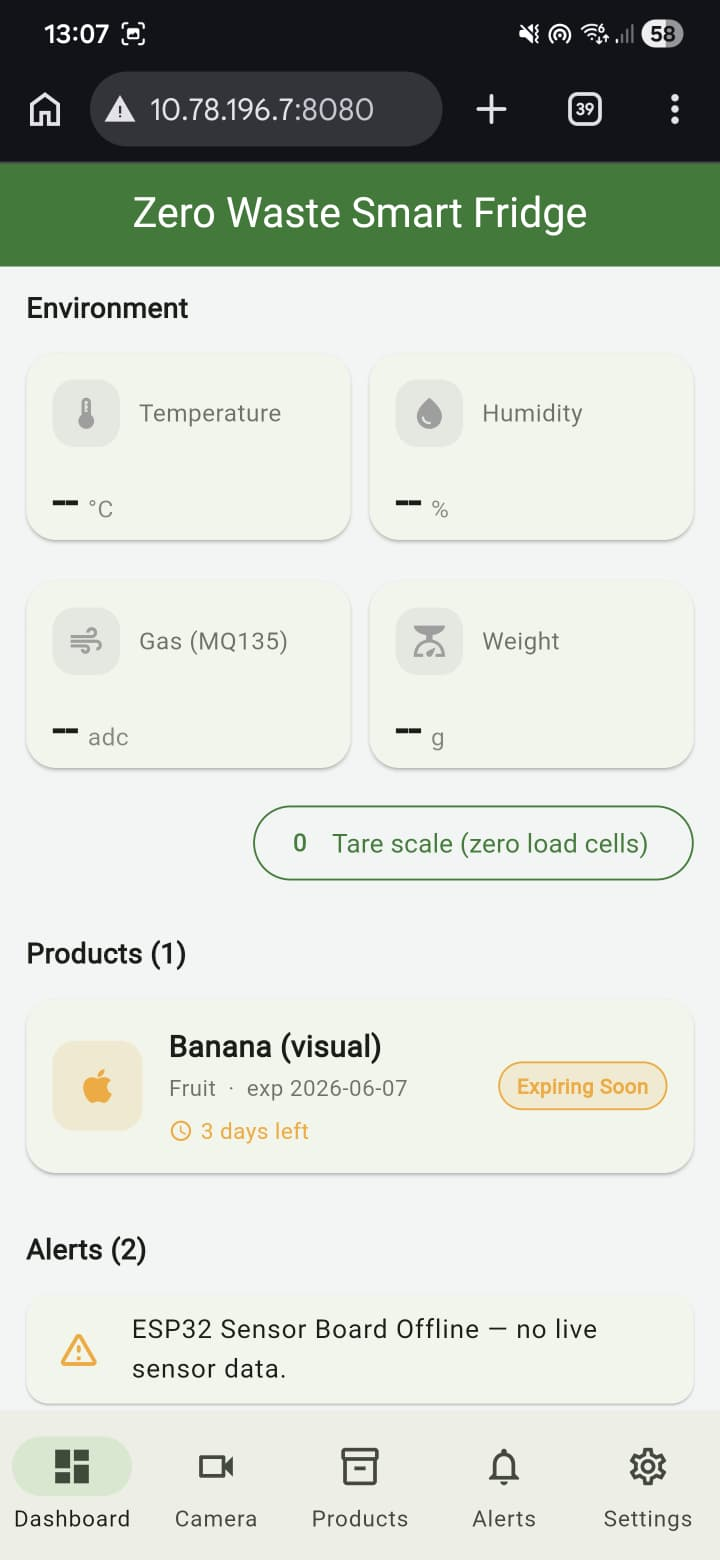
\includegraphics[width=0.30\textwidth]{../paper-assets/app-screens/07-app-dashboard.jpeg}
&
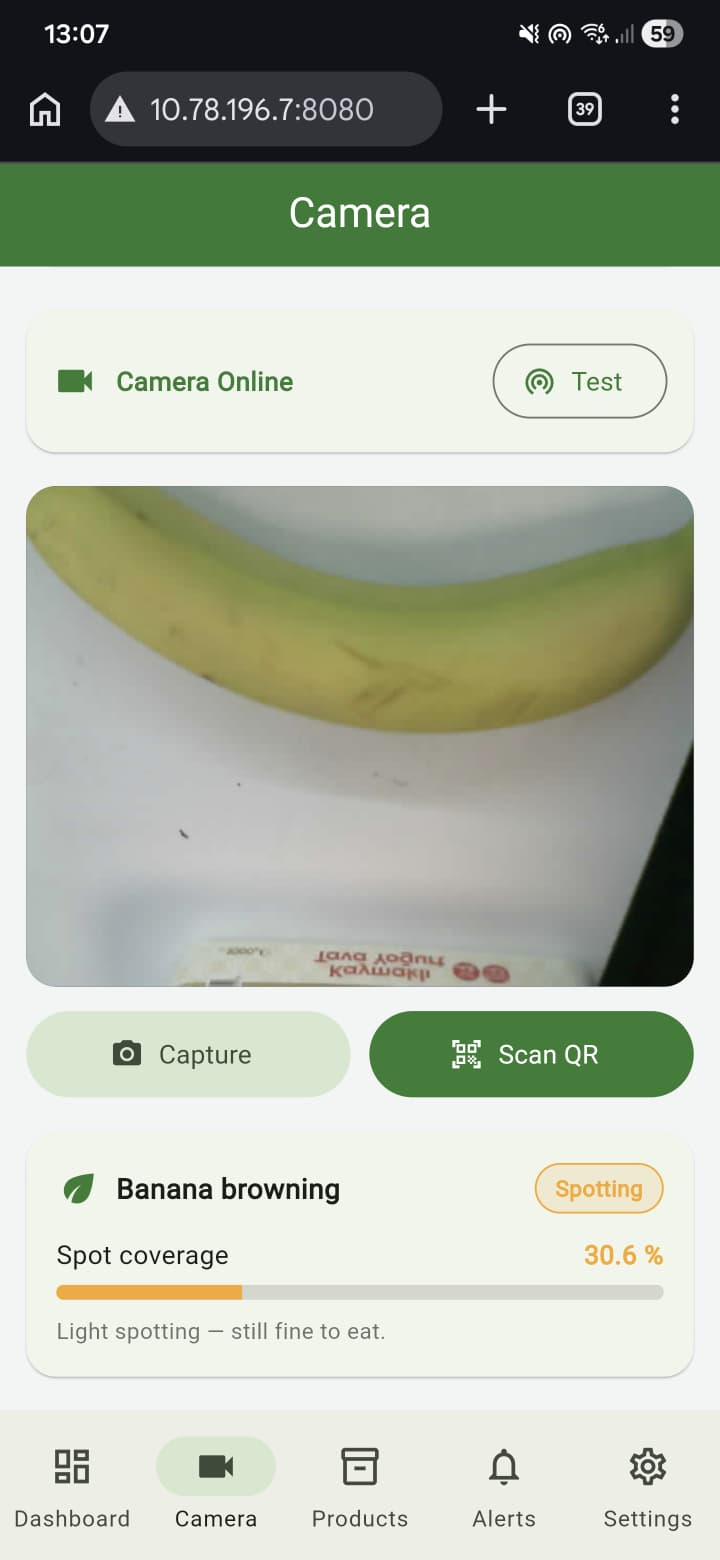
\includegraphics[width=0.30\textwidth]{../paper-assets/app-screens/05-app-camera-banana-spotting.jpeg}
\\
(a) Dashboard & (b) Camera --- live banana \\
\\
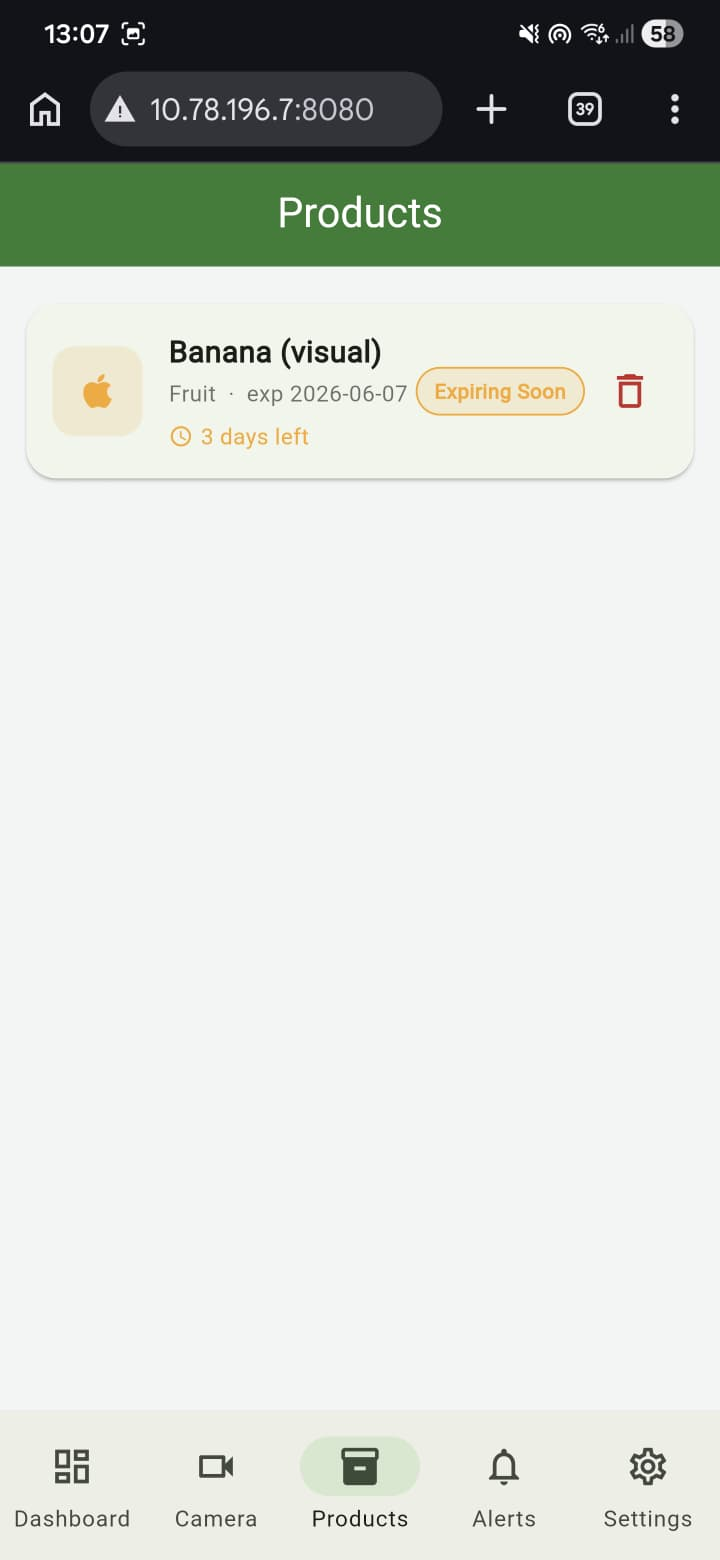
\includegraphics[width=0.30\textwidth]{../paper-assets/app-screens/06-app-products-banana.jpeg}
&
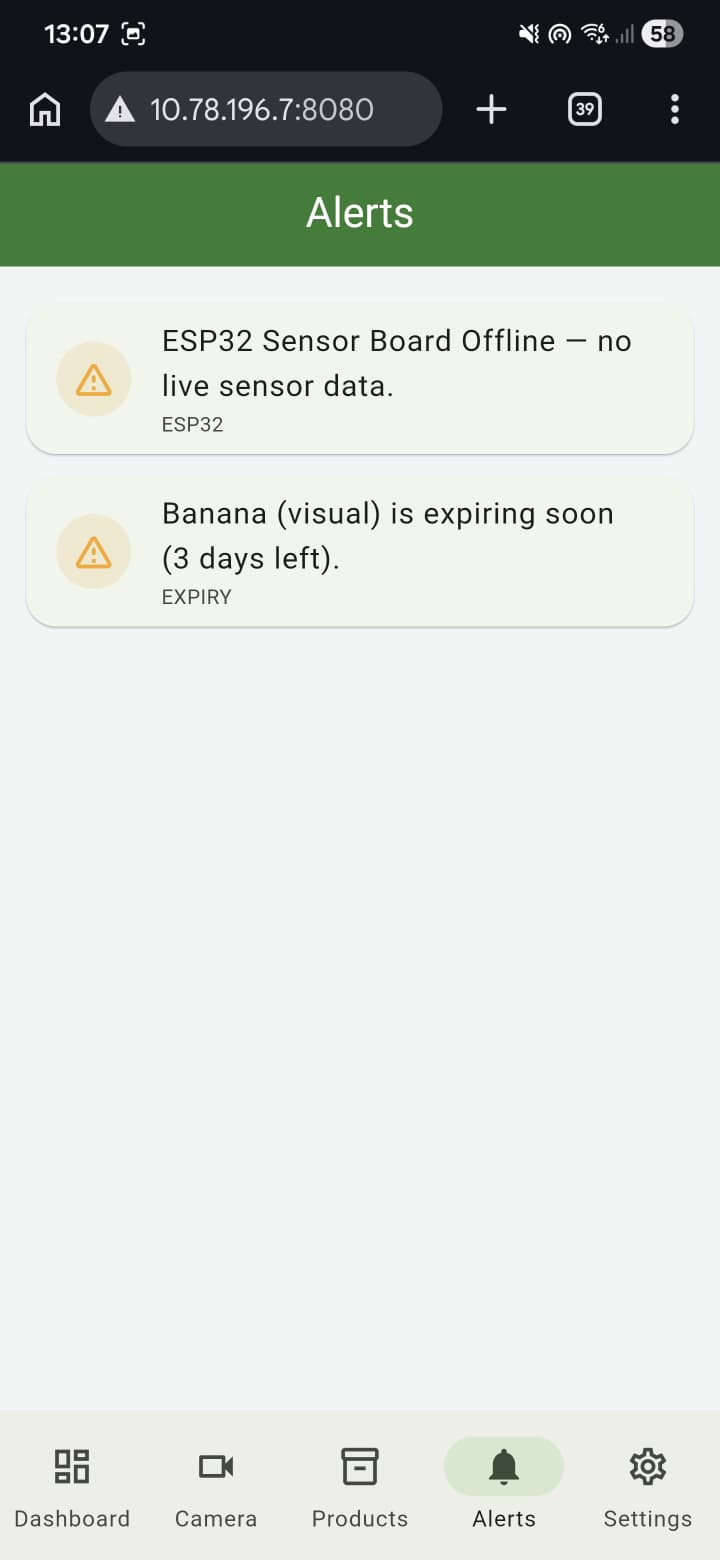
\includegraphics[width=0.30\textwidth]{../paper-assets/app-screens/04-app-alerts.jpeg}
\\
(c) Products & (d) Alerts \\
\\
\multicolumn{2}{c}{
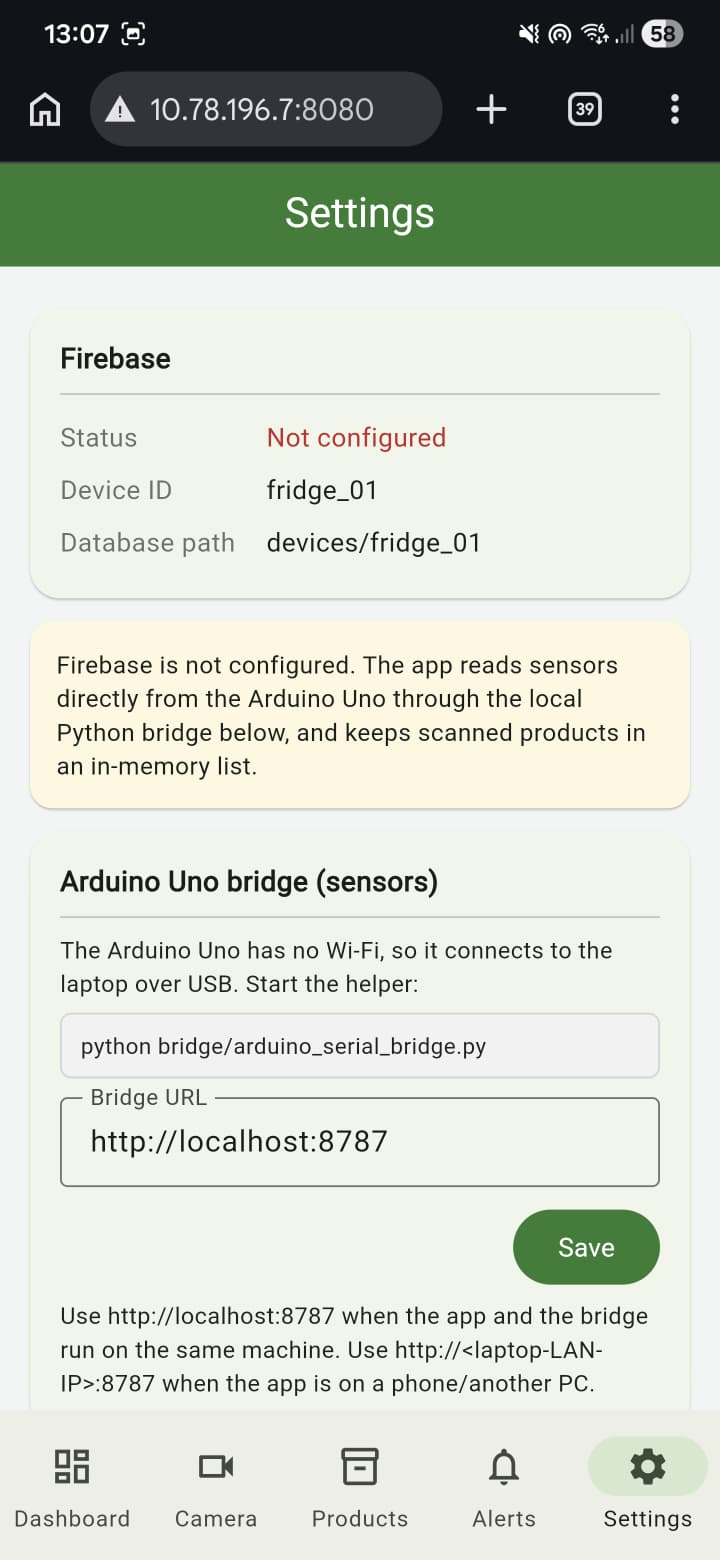
\includegraphics[width=0.30\textwidth]{../paper-assets/app-screens/08-app-settings.jpeg}}
\\
\multicolumn{2}{c}{(e) Settings} \\
\end{tabular}
\caption{Mobile application running during a demonstration session.
(a)~Dashboard with the four sensor cards, the registered Banana product,
and the active alert summary. (b)~Camera screen showing the live MJPEG
stream from the ESP32-CAM with a real banana in frame; the in-app
classifier reports 30.6\,\% spot coverage, labeled \emph{Spotting} ---
light spotting, still consumable. (c)~Products screen showing the
registered banana with a 3-day-until-expiration status band.
(d)~Alerts screen showing the automatically generated reminder and the
offline-sensor notice. (e)~Settings screen with the Firebase status,
the device identifier, and the bridge URL configuration field.}
\label{fig:app}
\end{figure*}

The \textbf{Dashboard} subscribes to the bridge's \texttt{/sensors}
endpoint via a one-second \texttt{Stream.periodic} timer, rebuilds the
four sensor cards when new readings arrive, and exposes the
\emph{Tare scale} button that issues a \texttt{POST /tare} command back
through the bridge.

The \textbf{Camera} screen displays the ESP32-CAM's MJPEG stream
through a small platform-specific widget (an \texttt{Image.network}
poll on the web target, an \texttt{HTTP-MJPEG} streaming widget on
Android) and runs the QR detection pipeline described in
Section~\ref{sec:algo-qr} on the corresponding JPEG captures fetched
from port 80.

The \textbf{Products} screen renders the in-memory product list
populated by the QR scanner. Each product card shows its expiration
status and a band color computed from the days remaining (Fresh,
Expiring Soon, or Expired).

The \textbf{Alerts} screen aggregates the alert engine's output,
which is rule-based: an alert is emitted when the bridge has not been
reachable for ten seconds, when a registered product's expiration is
within three days, when the cabinet's measured gas value rises sharply
relative to the smoothed baseline, or when the cabinet's temperature
exceeds a configurable threshold.

The \textbf{Settings} screen lets the user enter the bridge URL and
the ESP32-CAM's IP address, save them to local storage, and observe
the Firebase configuration status (a placeholder; the deployed
prototype intentionally operates in \emph{in-memory mode} without a
back end so that it remains usable in environments without a Firebase
project).
